\section{Mathematical Demonstrations} 
\subsection{Movement in R3} \label{movement-in-r3}

Property of Prof. Oliver Augenstein. This is a scanned pdf, therefore the design might be inconsistent with the other parts of the thesis.

\begin{figure}[h!]
	\centering
	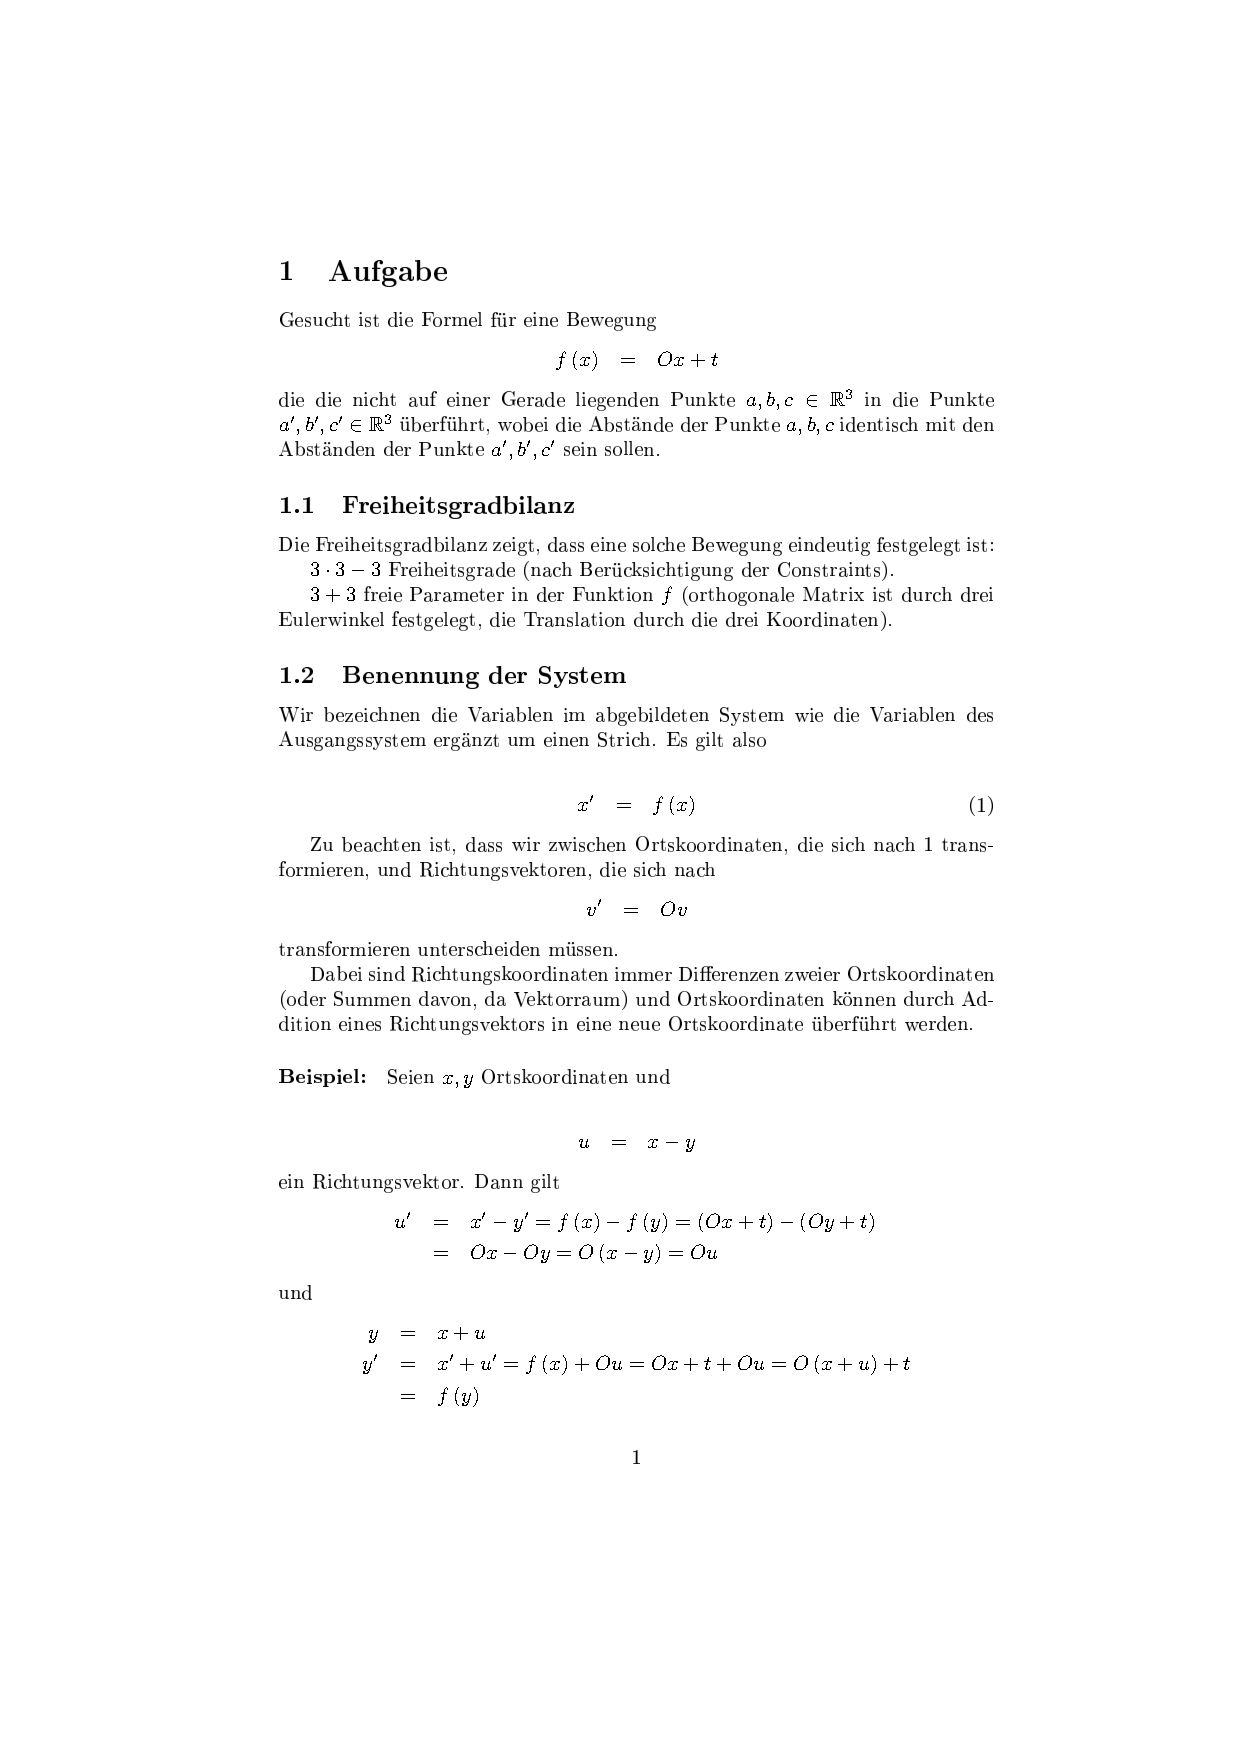
\includegraphics[width=0.8\textwidth]{movement_in_r3_1}
\end{figure}
\newpage
\begin{figure}[h!]
	\centering
	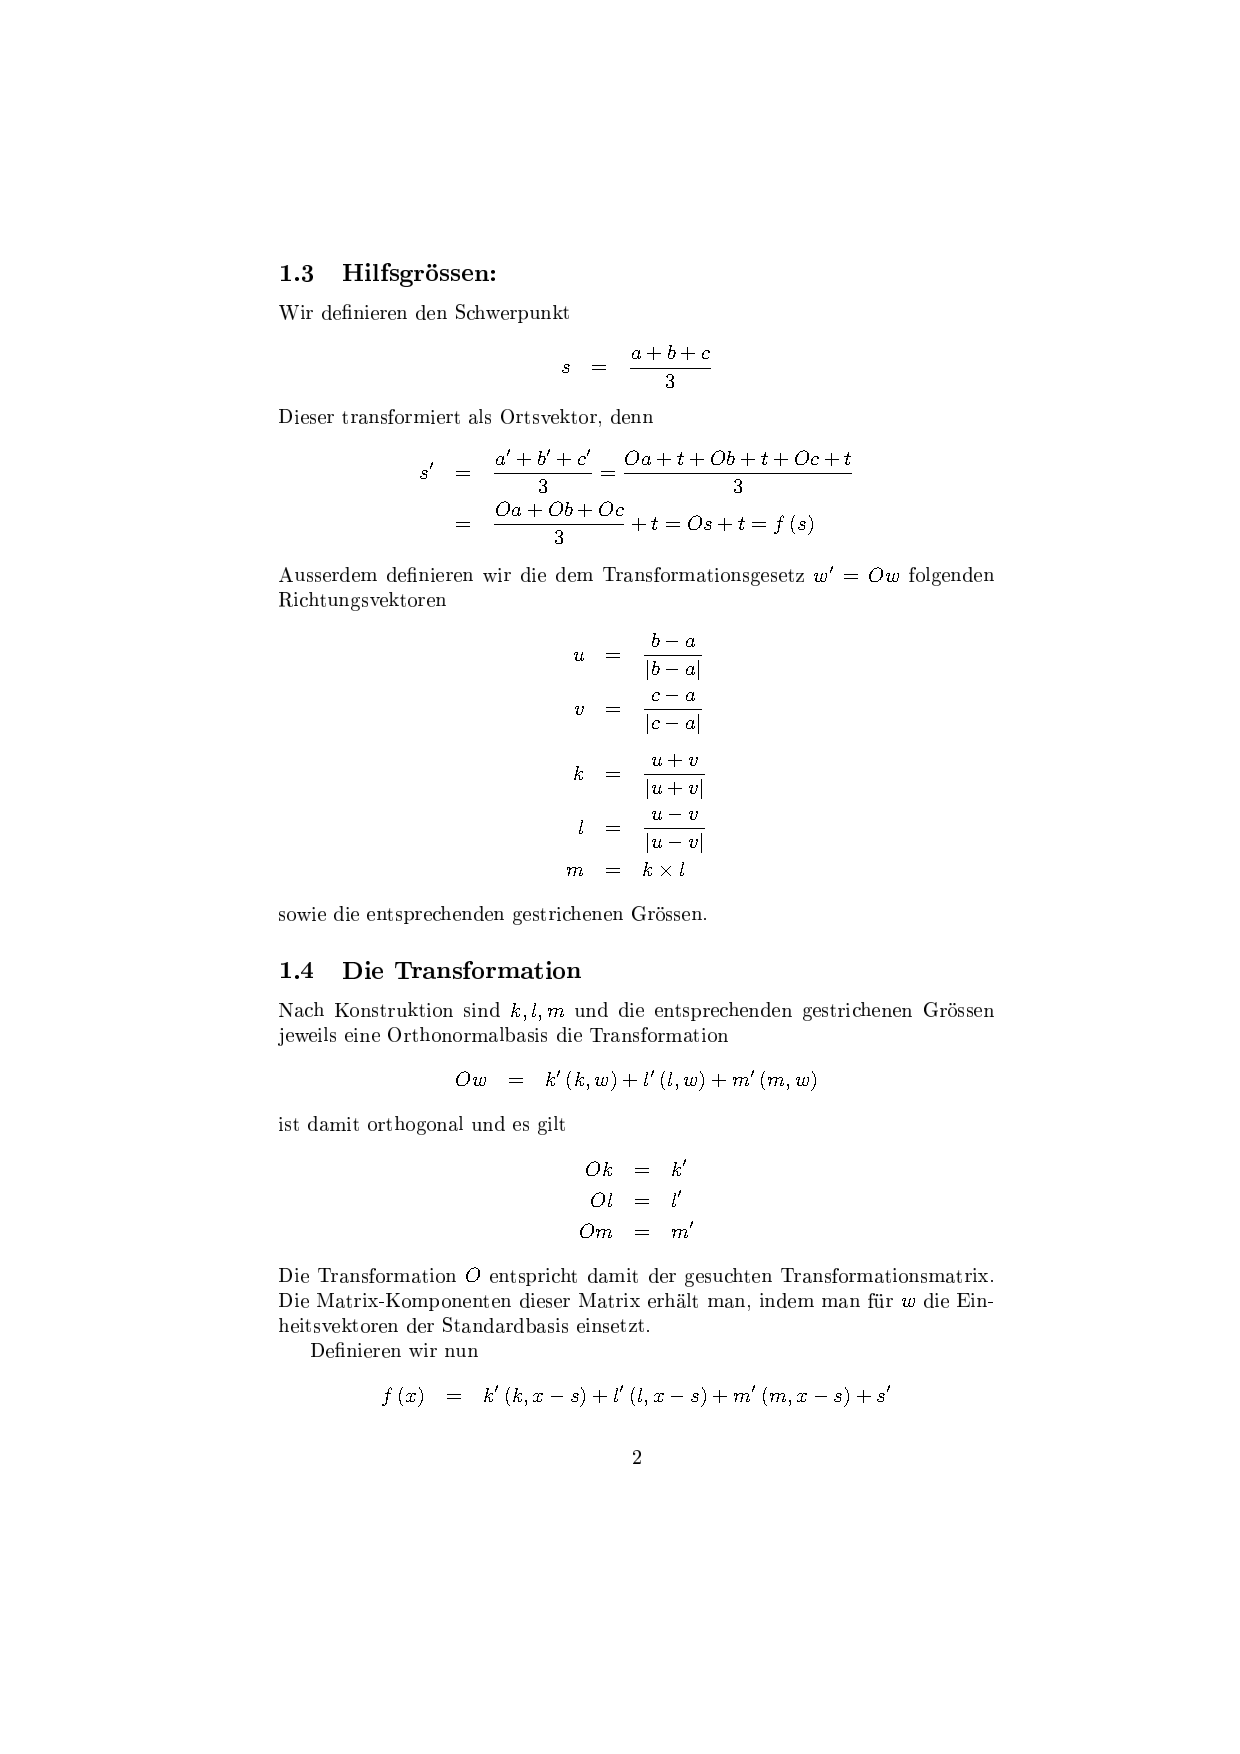
\includegraphics[width=0.8\textwidth]{movement_in_r3_2}
\end{figure}
\newpage
\begin{figure}[h!]
	\centering
	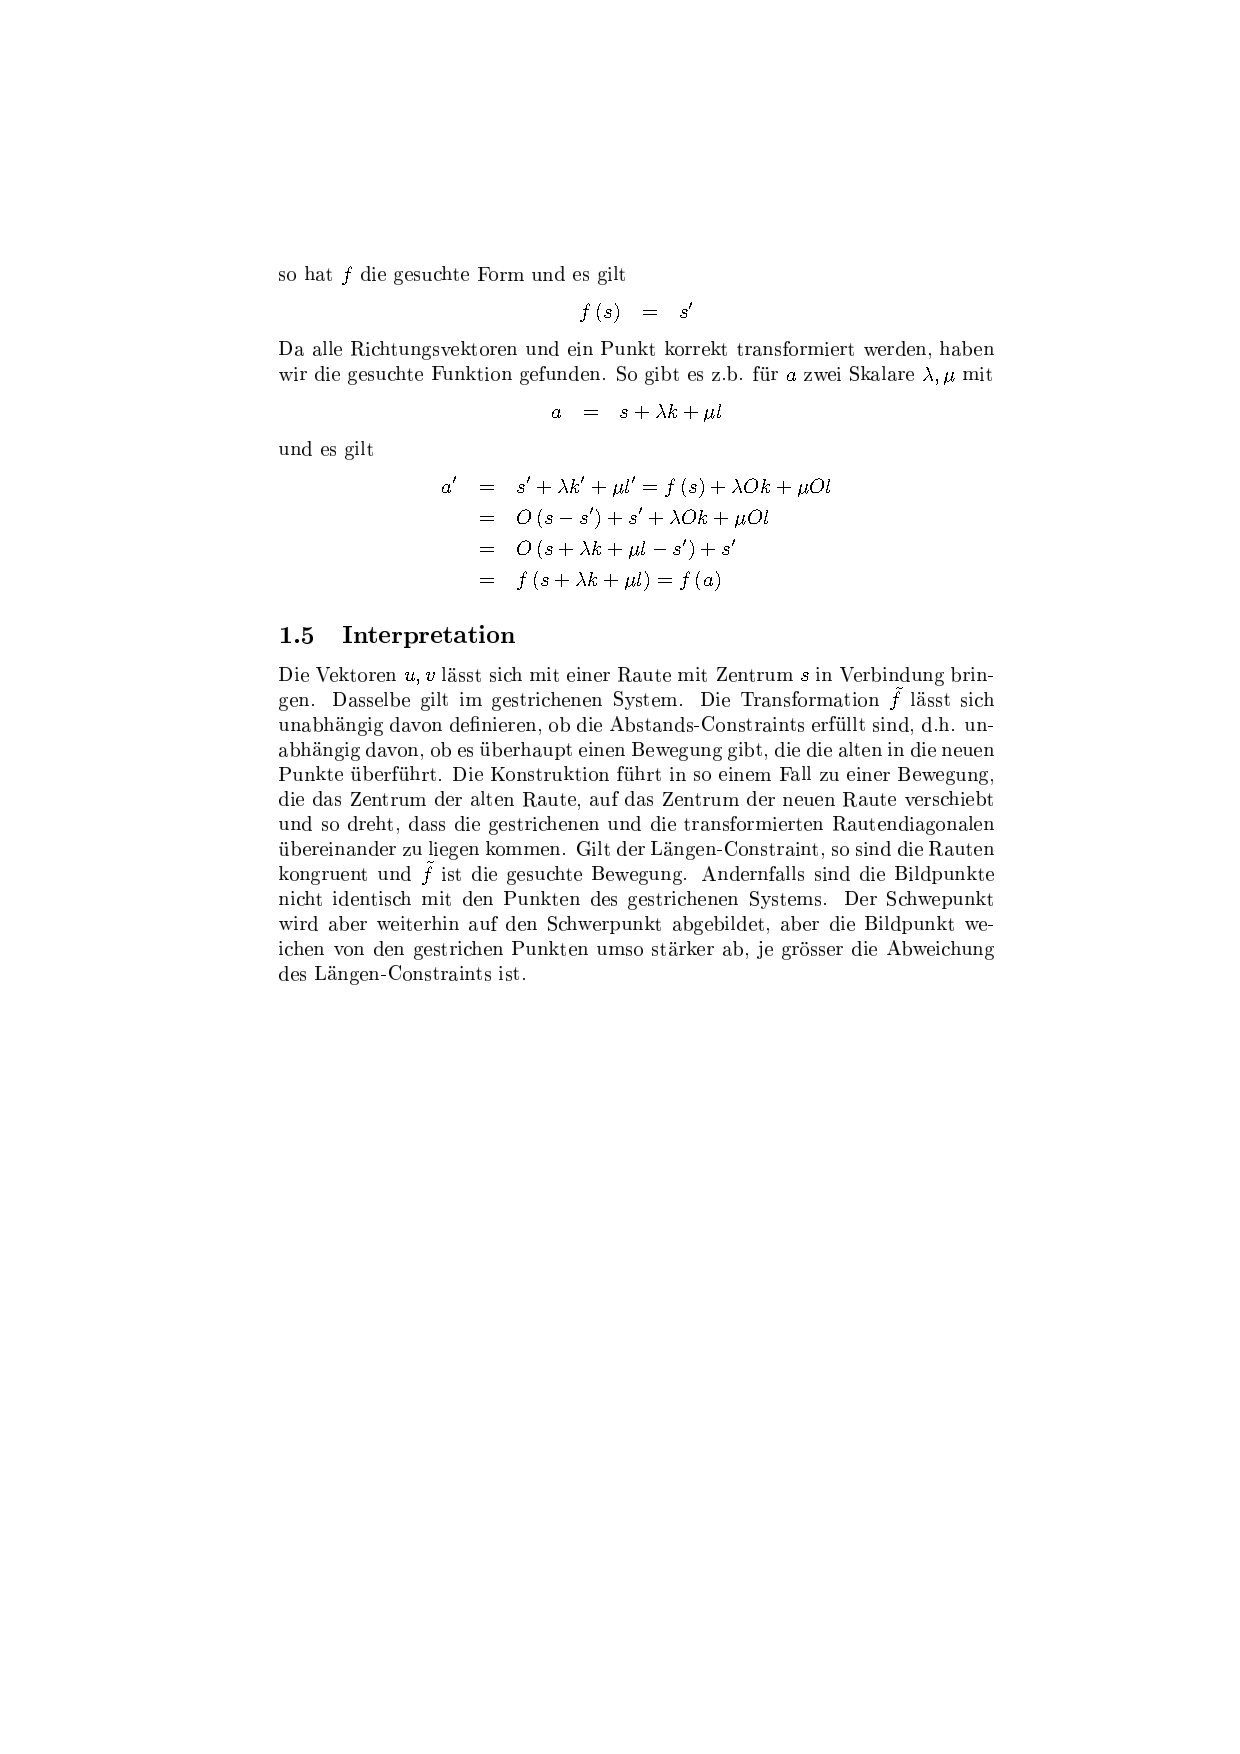
\includegraphics[width=0.8\textwidth]{movement_in_r3_3}
\end{figure}
